\chapter{Linear Lists}\label{ch04:linear-lists}

\section{Introduction}

> \textbf{Complete compilable implementations of the data structures in this chapter are in \texttt{code/}.}

\section{Array-Based Lists}

\subsection{The Linear List Abstract Data Type}

A \textbf{linear list} (also called a sequence or vector) is an ordered collection of elements where each element has a position. The positions are numbered from 0 (or 1, depending on convention). We use 0-based indexing throughout this book.

\textbf{Operations.} A linear list ADT supports these core operations:

\begin{itemize}
\item \textbf{get(index)} — return the element at position index
\item \textbf{set(index, value)} — replace the element at position index
\item \textbf{insert(index, value)} — insert value at position index, shifting subsequent elements right
\item \textbf{erase(index)} — remove the element at position index, shifting subsequent elements left
\item \textbf{size()} — return the number of elements
\item \textbf{empty()} — return true iff size is 0
\item \textbf{push\_back(value)} — append to the end (convenience)
\item \textbf{pop\_back()} — remove from the end (convenience)
\item \textbf{clear()} — remove all elements
\end{itemize}

\textbf{Applications.} Linear lists appear everywhere:
\begin{itemize}
\item A text editor stores lines in a list
\item A music player stores a playlist
\item A spreadsheet stores rows of cells
\item An image editor stores layers
\end{itemize}

\subsection{Array Representation}

The simplest way to represent a linear list is with a fixed-size array. We allocate an array large enough to hold the maximum number of elements and track the current number of elements.

\begin{figure}[ht]
\centering
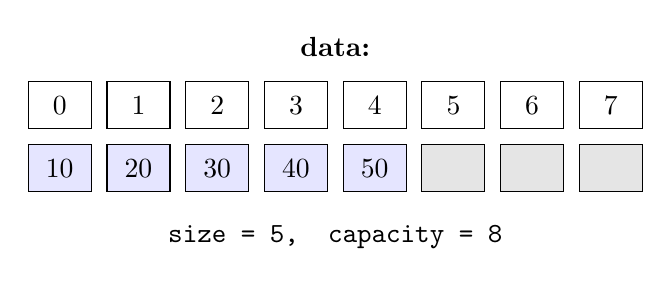
\begin{tikzpicture}
\begin{scope}[every node/.style={draw,minimum width=0.8cm,minimum height=0.6cm}]
  \node (i0) at (0,0.8) {0};
  \node (i1) at (1,0.8) {1};
  \node (i2) at (2,0.8) {2};
  \node (i3) at (3,0.8) {3};
  \node (i4) at (4,0.8) {4};
  \node (i5) at (5,0.8) {5};
  \node (i6) at (6,0.8) {6};
  \node (i7) at (7,0.8) {7};
  \node[fill=blue!10] (d0) at (0,0) {10};
  \node[fill=blue!10] (d1) at (1,0) {20};
  \node[fill=blue!10] (d2) at (2,0) {30};
  \node[fill=blue!10] (d3) at (3,0) {40};
  \node[fill=blue!10] (d4) at (4,0) {50};
  \node[fill=gray!20] (d5) at (5,0) {};
  \node[fill=gray!20] (d6) at (6,0) {};
  \node[fill=gray!20] (d7) at (7,0) {};
\end{scope}
\node[above] at (3.5,1.3) {\textbf{data:}};
\node[below] at (3.5,-0.6) {\texttt{size = 5,\ \ capacity = 8}};
\end{tikzpicture}
\end{figure}

\textbf{Fixed-Capacity List.}

\begin{lstlisting}[language=C++]
template <typename T>
class array_list {
public:
    using value_type = T;
    using size_type = std::size_t;
    using reference = T&;
    using const_reference = const T&;

    explicit array_list(size_type capacity)
        : capacity_(capacity), size_(0), data_(std::make_unique<T[]>(capacity)) {}

    size_type size() const noexcept { return size_; }
    bool empty() const noexcept { return size_ == 0; }
    size_type capacity() const noexcept { return capacity_; }

    reference operator[](size_type index) {
        check_index(index);
        return data_[index];
    }

    const_reference operator[](size_type index) const {
        check_index(index);
        return data_[index];
    }

    void push_back(const T& value) {
        if (size_ >= capacity_) throw std::overflow_error("list is full");
        data_[size_++] = value;
    }

    void pop_back() {
        if (empty()) throw std::underflow_error("list is empty");
        --size_;
    }

    void insert(size_type index, const T& value) {
        if (size_ >= capacity_) throw std::overflow_error("list is full");
        if (index > size_) throw std::out_of_range("index out of range");
        for (size_type i = size_; i > index; --i) {
            data_[i] = data_[i - 1];
        }
        data_[index] = value;
        ++size_;
    }

    void erase(size_type index) {
        if (index >= size_) throw std::out_of_range("index out of range");
        for (size_type i = index; i < size_ - 1; ++i) {
            data_[i] = data_[i + 1];
        }
        --size_;
    }

    void clear() noexcept { size_ = 0; }

private:
    void check_index(size_type index) const {
        if (index >= size_) throw std::out_of_range("index out of range");
    }

    size_type capacity_;
    size_type size_;
    std::unique_ptr<T[]> data_;
};
\end{lstlisting}

This implementation has a serious limitation: the capacity is fixed at construction time. If we need more space, we fail.

\subsection{Dynamic Array (Resizable Array)}

The solution is to grow the array when it becomes full. This is the strategy used by \texttt{std::vector}.

\textbf{Growth strategy.} When a \texttt{push\_back} finds the array full:
\begin{enumerate}
\item Allocate a new array of larger capacity (typically 2$\times $ the old size)
\item Move all elements from the old array to the new one
\item Deallocate the old array
\item Insert the new element
\end{enumerate}

\textbf{Implementation.}

\begin{lstlisting}[language=C++]
template <typename T>
class dynamic_array_list {
public:
    using value_type = T;
    using size_type = std::size_t;
    using reference = T&;
    using const_reference = const T&;
    using iterator = T*;
    using const_iterator = const T*;

    static constexpr size_type default_capacity = 4;

    dynamic_array_list() : size_(0), capacity_(default_capacity),
                           data_(std::make_unique<T[]>(default_capacity)) {}

    dynamic_array_list(std::initializer_list<T> init)
        : size_(init.size()), capacity_(init.size()),
          data_(std::make_unique<T[]>(init.size())) {
        std::copy(init.begin(), init.end(), data_.get());
    }

    dynamic_array_list(const dynamic_array_list& other)
        : size_(other.size_), capacity_(other.capacity_),
          data_(std::make_unique<T[]>(other.capacity_)) {
        std::copy(other.data_.get(), other.data_.get() + size_, data_.get());
    }

    dynamic_array_list& operator=(const dynamic_array_list& other) {
        if (this != &other) {
            auto new_data = std::make_unique<T[]>(other.capacity_);
            std::copy(other.data_.get(), other.data_.get() + other.size_, new_data.get());
            size_ = other.size_;
            capacity_ = other.capacity_;
            data_ = std::move(new_data);
        }
        return *this;
    }

    dynamic_array_list(dynamic_array_list&&) = default;
    dynamic_array_list& operator=(dynamic_array_list&&) = default;

    reference operator[](size_type index) {
        check_index(index);
        return data_[index];
    }
    const_reference operator[](size_type index) const {
        check_index(index);
        return data_[index];
    }

    reference at(size_type index) {
        if (index >= size_) throw std::out_of_range("index out of range");
        return data_[index];
    }
    const_reference at(size_type index) const {
        if (index >= size_) throw std::out_of_range("index out of range");
        return data_[index];
    }

    reference front() { return data_[0]; }
    const_reference front() const { return data_[0]; }
    reference back() { return data_[size_ - 1]; }
    const_reference back() const { return data_[size_ - 1]; }

    size_type size() const noexcept { return size_; }
    size_type capacity() const noexcept { return capacity_; }
    bool empty() const noexcept { return size_ == 0; }

    void reserve(size_type new_capacity) {
        if (new_capacity > capacity_) {
            grow(new_capacity);
        }
    }

    void push_back(const T& value) {
        if (size_ >= capacity_) grow(2 * capacity_);
        data_[size_++] = value;
    }

    void push_back(T&& value) {
        if (size_ >= capacity_) grow(2 * capacity_);
        data_[size_++] = std::move(value);
    }

    template <typename... Args>
    reference emplace_back(Args&&... args) {
        if (size_ >= capacity_) grow(2 * capacity_);
        data_[size_] = T(std::forward<Args>(args)...);
        return data_[size_++];
    }

    void pop_back() {
        if (empty()) throw std::underflow_error("list is empty");
        --size_;
    }

    void insert(size_type index, const T& value) {
        if (index > size_) throw std::out_of_range("index out of range");
        if (size_ >= capacity_) grow(2 * capacity_);
        for (size_type i = size_; i > index; --i) {
            data_[i] = std::move(data_[i - 1]);
        }
        data_[index] = value;
        ++size_;
    }

    void erase(size_type index) {
        if (index >= size_) throw std::out_of_range("index out of range");
        for (size_type i = index; i < size_ - 1; ++i) {
            data_[i] = std::move(data_[i + 1]);
        }
        --size_;
    }

    void clear() noexcept { size_ = 0; }

    void shrink_to_fit() {
        if (size_ < capacity_) {
            auto new_data = std::make_unique<T[]>(size_);
            std::move(data_.get(), data_.get() + size_, new_data.get());
            capacity_ = size_;
            data_ = std::move(new_data);
        }
    }

    iterator begin() noexcept { return data_.get(); }
    const_iterator begin() const noexcept { return data_.get(); }
    iterator end() noexcept { return data_.get() + size_; }
    const_iterator end() const noexcept { return data_.get() + size_; }

private:
    void check_index(size_type index) const {
        if (index >= size_) throw std::out_of_range("index out of range");
    }

    void grow(size_type new_capacity) {
        auto new_data = std::make_unique<T[]>(new_capacity);
        std::move(data_.get(), data_.get() + size_, new_data.get());
        capacity_ = new_capacity;
        data_ = std::move(new_data);
    }

    size_type size_;
    size_type capacity_;
    std::unique_ptr<T[]> data_;
};
\end{lstlisting}

\textbf{Step-by-step walkthrough.} Consider the sequence of operations on an initially empty list:

\textbf{push\_back(10):} size=0, capacity=4. Insert data[0]=10, size=1.
\begin{lstlisting}[language=Java]
    [10 | _ | _ | _ ]
     0    1   2   3
\end{lstlisting}

\textbf{push\_back(20):} size=1, capacity=4. Insert data[1]=20, size=2.
\begin{lstlisting}[language=Java]
    [10 | 20 | _ | _ ]
\end{lstlisting}

\textbf{push\_back(30), push\_back(40):} size=4.
\begin{lstlisting}[language=Java]
    [10 | 20 | 30 | 40]
\end{lstlisting}

\textbf{push\_back(50):} size=4 $\ge $ capacity=4 $\to $ grow to 8. Copy elements.
\begin{lstlisting}[language=Java]
    [10 | 20 | 30 | 40 | 50 | _ | _ | _ ]
\end{lstlisting}

\textbf{insert(2, 25):} size=5, capacity=8. Shift elements at indices 2,3,4 right.
\begin{lstlisting}[language=Java]
    [10 | 20 | 25 | 30 | 40 | 50 | _ | _ ]
\end{lstlisting}

\textbf{erase(4):} size=6. Shift elements at indices 5,6 left.
\begin{lstlisting}[language=Java]
    [10 | 20 | 25 | 30 | 50 | _ | _ | _ ]
    size=5
\end{lstlisting}

\subsection{Complexity Analysis}

\begin{center}
\begin{tabular}{ccc}
\toprule
Operation & Fixed Array & Dynamic Array (amortized) \\
\texttt{operator[]} & O(1) & O(1) \\
\texttt{push\_back} & O(1) & O(1) amortized \\
\texttt{pop\_back} & O(1) & O(1) \\
\texttt{insert} at front & O(n) & O(n) \\
\texttt{insert} at back & O(1) & O(1) amortized \\
\texttt{insert} at middle & O(n) & O(n) \\
\texttt{erase} at front & O(n) & O(n) \\
\texttt{erase} at back & O(1) & O(1) \\
\texttt{erase} at middle & O(n) & O(n) \\
Space (overhead) & O(capacity) & O(size) \\

\bottomrule
\end{tabular}
\end{center}
Why is \texttt{push\_back} O(1) amortized? The resize copies n elements every n insertions. The total cost of n insertions is at most 3n: n unit-cost insertions plus at most 2n element copies across all resizes (as shown in Chapter 2).

\subsection{Application: Polynomial Arithmetic}

We can represent a polynomial using an array list of coefficients. The index is the exponent; the value is the coefficient.

\begin{lstlisting}[language=C++]
class polynomial {
public:
    polynomial() : coeff_(1) {}  // zero polynomial

    void set_coefficient(int exponent, double coefficient) {
        while (static_cast<int>(coeff_.size()) <= exponent) {
            coeff_.push_back(0.0);
        }
        coeff_[exponent] = coefficient;
    }

    double evaluate(double x) const {
        double result = 0.0;
        double power = 1.0;
        for (size_t i = 0; i < coeff_.size(); ++i) {
            result += coeff_[i] * power;
            power *= x;
        }
        return result;
    }

    double coefficient(int exponent) const {
        if (exponent >= static_cast<int>(coeff_.size())) return 0.0;
        return coeff_[exponent];
    }

    int degree() const {
        for (int i = static_cast<int>(coeff_.size()) - 1; i >= 0; --i) {
            if (coeff_[i] != 0.0) return i;
        }
        return -1;  // zero polynomial
    }

private:
    dynamic_array_list<double> coeff_;
};
\end{lstlisting}

\textbf{Example.} Polynomial: 3x$^{5}$ - 2x$^{2}$ + 7

\begin{lstlisting}[language=Java]
coeff_ = [7, 0, -2, 0, 0, 3]
index:    0  1   2  3  4  5

evaluate at x = 2:
7 + 0$\cdot$2 + (-2)$\cdot$4 + 0$\cdot$8 + 0$\cdot$16 + 3$\cdot$32
= 7 - 8 + 96 = 95
\end{lstlisting}

\subsection{Application: Image Editor Layer Stack}

A layer stack in an image editor is a linear list of layers. Adding a layer appends to the top. Deleting a layer removes it by index. Reordering moves a layer from one index to another.

\begin{lstlisting}[language=C++]
struct layer {
    std::string name;
    bool visible = true;
    float opacity = 1.0f;
};

using layer_stack = dynamic_array_list<layer>;

void reorder_layer(layer_stack& stack, size_t from, size_t to) {
    layer l = std::move(stack[from]);
    stack.erase(from);
    stack.insert(to, std::move(l));
}
\end{lstlisting}

\subsection{STL Connection: std::vector}

Our \texttt{dynamic\_array\_list} closely mirrors \texttt{std::vector}. The standard library version adds:
\begin{itemize}
\item \textbf{Allocator support} — custom memory allocation strategies
\item \textbf{\texttt{data()}} — raw pointer access
\item \textbf{\texttt{resize(n)}} — change size, default-construct or destroy elements
\item \textbf{\texttt{assign}} — replace all elements
\item \textbf{Comparison operators} — lexicographic comparison
\item \textbf{\texttt{swap}} — O(1) exchange of two vectors
\item \textbf{Exception safety guarantees} — strong guarantee for most operations
\end{itemize}

\begin{lstlisting}[language=C++]
std::vector<int> v = {1, 2, 3};
v.push_back(4);
v.insert(v.begin(), 0);
std::sort(v.begin(), v.end());
\end{lstlisting}

The fundamental design is the same: a contiguous array that grows geometrically.

\bigskip

\section{Linked Lists}

Array-based lists have a fundamental limitation: inserting or erasing elements in the middle requires shifting O(n) elements. A \textbf{linked list\index{linked list}} avoids this by storing elements in separately allocated \textbf{nodes} connected by pointers.

Each node contains:
\begin{itemize}
\item A \textbf{data} field holding the element
\item A \textbf{next} pointer to the next node (and optionally a \textbf{prev} pointer for doubly linked\index{doubly linked} lists)
\end{itemize}

\subsection{Singly Linked List (Chain)}

A singly linked\index{singly linked} list connects nodes in one direction:

\begin{figure}[ht]
\centering
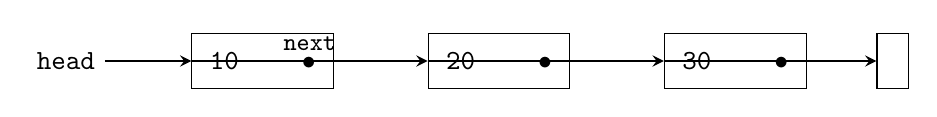
\begin{tikzpicture}
\tikzstyle{nodebox}=[draw,rectangle,minimum width=1.8cm,minimum height=0.7cm,inner sep=2pt]
\tikzstyle{nullbox}=[draw,rectangle,minimum width=0.4cm,minimum height=0.7cm,inner sep=2pt]
\node (headlabel) at (0,0.5) {\texttt{head}};
\node[nodebox] (n1) at (2.5,0.5) {\texttt{10}\hspace{0.8cm}\texttt{$\bullet$}};
\node[nodebox] (n2) at (5.5,0.5) {\texttt{20}\hspace{0.8cm}\texttt{$\bullet$}};
\node[nodebox] (n3) at (8.5,0.5) {\texttt{30}\hspace{0.8cm}\texttt{$\bullet$}};
\node[nullbox] (null) at (10.5,0.5) {$\varnothing$};
\draw[->,>=stealth,thick] (headlabel.east) -- (n1.west);
\draw[->,>=stealth,thick] (1.6,0.5) -- node[above]{\small\texttt{next}} (n2.west);
\draw[->,>=stealth,thick] (4.6,0.5) -- (n3.west);
\draw[->,>=stealth,thick] (7.6,0.5) -- (null.west);
\end{tikzpicture}
\end{figure}

\textbf{Node structure.}

\begin{lstlisting}[language=C++]
template <typename T>
struct node {
    T data;
    std::unique_ptr<node> next;

    explicit node(const T& value) : data(value), next(nullptr) {}
    explicit node(T&& value) : data(std::move(value)), next(nullptr) {}
};
\end{lstlisting}

We use \texttt{std::unique\_ptr} for owning pointers — when a node is destroyed, its \texttt{next} chain is automatically freed.

\textbf{Implementation.}

\begin{lstlisting}[language=C++]
template <typename T>
class linked_list {
public:
    using value_type = T;
    using size_type = std::size_t;
    using reference = T&;
    using const_reference = const T&;

    linked_list() = default;

    linked_list(std::initializer_list<T> init) {
        for (const auto& value : init) {
            push_back(value);
        }
    }

    linked_list(const linked_list& other) {
        node<T>* current = other.head_.get();
        node<T>** tail = &head_;
        while (current) {
            *tail = std::make_unique<node<T>>(current->data);
            tail = &(*tail)->next;
            current = current->next.get();
        }
        size_ = other.size_;
    }

    linked_list& operator=(const linked_list& other) {
        if (this != &other) {
            linked_list temp(other);
            std::swap(head_, temp.head_);
            std::swap(size_, temp.size_);
        }
        return *this;
    }

    linked_list(linked_list&&) = default;
    linked_list& operator=(linked_list&&) = default;

    reference front() {
        if (empty()) throw std::underflow_error("list is empty");
        return head_->data;
    }
    const_reference front() const {
        if (empty()) throw std::underflow_error("list is empty");
        return head_->data;
    }

    size_type size() const noexcept { return size_; }
    bool empty() const noexcept { return size_ == 0; }

    void push_front(const T& value) {
        auto new_node = std::make_unique<node<T>>(value);
        node<T>* raw_node = new_node.get();
        new_node->next = std::move(head_);
        head_ = std::move(new_node);
        if (!tail_) tail_ = raw_node;
        ++size_;
    }

    void push_front(T&& value) {
        auto new_node = std::make_unique<node<T>>(std::move(value));
        new_node->next = std::move(head_);
        head_ = std::move(new_node);
        ++size_;
    }

    void push_back(const T& value) {
        auto new_node = std::make_unique<node<T>>(value);
        node<T>* raw_node = new_node.get();
        if (!head_) {
            head_ = std::move(new_node);
        } else {
            tail_->next = std::move(new_node);
        }
        tail_ = raw_node;
        ++size_;
    }

    void pop_front() {
        if (empty()) throw std::underflow_error("list is empty");
        head_ = std::move(head_->next);
        if (!head_) tail_ = nullptr;
        --size_;
    }

    void clear() noexcept {
        head_.reset();
        size_ = 0;
    }

    reference operator[](size_type index) {
        node<T>* current = head_.get();
        for (size_type i = 0; i < index; ++i) {
            current = current->next.get();
        }
        return current->data;
    }

    class iterator {
    public:
        using iterator_category = std::forward_iterator_tag;
        using value_type = T;
        using difference_type = std::ptrdiff_t;
        using pointer = T*;
        using reference = T&;

        iterator(node<T>* ptr) : ptr_(ptr) {}

        reference operator*() const { return ptr_->data; }
        pointer operator->() const { return &ptr_->data; }
        iterator& operator++() { ptr_ = ptr_->next.get(); return *this; }
        iterator operator++(int) { iterator tmp = *this; ++(*this); return tmp; }
        bool operator==(const iterator& other) const { return ptr_ == other.ptr_; }
        bool operator!=(const iterator& other) const { return ptr_ != other.ptr_; }

    private:
        node<T>* ptr_;
    };

    iterator begin() noexcept { return iterator(head_.get()); }
    iterator end() noexcept { return iterator(nullptr); }

private:
    node<T>** get_tail_ptr() {
        node<T>** p = &head_;
        while (*p) p = &(*p)->next;
        return p;
    }

    std::unique_ptr<node<T>> head_;
    node<T>* tail_ = nullptr;
    size_type size_ = 0;
};
\end{lstlisting}

\textbf{Step-by-step walkthrough.} Building list L = {10, 20, 30}:

\textbf{Step 1: push\_back(10)}
\begin{lstlisting}[language=Java]
head  ->  [10 | /]
\end{lstlisting}

\textbf{Step 2: push\_back(20)}
\begin{lstlisting}[language=Java]
head  ->  [10 | $\cdot$]  ->  [20 | /]
\end{lstlisting}

\textbf{Step 3: push\_back(30)}
\begin{lstlisting}[language=Java]
head  ->  [10 | $\cdot$]  ->  [20 | $\cdot$]  ->  [30 | /]
\end{lstlisting}

\textbf{Step 4: pop\_front()}
\begin{lstlisting}[language=Java]
head  ->  [20 | $\cdot$]  ->  [30 | /]
// (10 is automatically freed since unique_ptr goes out of scope)
\end{lstlisting}

\subsection{Complexity Analysis}

\begin{center}
\begin{tabular}{ccc}
\toprule
Operation & Array List & Singly Linked List \\
\texttt{operator[]} & O(1) & O(n) \\
\texttt{push\_front} & O(n) & O(1) \\
\texttt{push\_back} & O(1) amortized & O(1) with tail ptr \\
\texttt{pop\_front} & O(n) & O(1) \\
\texttt{pop\_back} & O(1) & O(n) \\
\texttt{insert} at known position & O(n) & O(1) once positioned \\
space overhead & O(1) per list & O(n) for pointers \\

\bottomrule
\end{tabular}
\end{center}
\textbf{Key tradeoff:} Linked lists sacrifice O(1) random access for O(1) front insertions/deletions.

\subsection{Doubly Linked List}

A doubly linked list has prev and next pointers, enabling O(1) deletion at both ends and bidirectional traversal.

\begin{lstlisting}[language=Java]
null  <-  [10 | $\cdot$ | $\cdot$] <-> [20 | $\cdot$ | $\cdot$] <-> [30 | / | $\cdot$]  ->  null
\end{lstlisting}

\begin{lstlisting}[language=C++]
template <typename T>
struct dnode {
    T data;
    std::unique_ptr<dnode> next;
    dnode* prev;

    explicit dnode(const T& value) : data(value), next(nullptr), prev(nullptr) {}
};
\end{lstlisting}

\textbf{Doubly linked list with sentinel.} A sentinel (dummy header node) simplifies edge cases — every real node has a non-null predecessor:

\begin{lstlisting}[language=C++]
template <typename T>
class doubly_linked_list {
public:
    doubly_linked_list() : size_(0) {
        head_ = std::make_unique<dnode<T>>(T());
        tail_ = head_.get();
    }

    void push_front(const T& value) {
        auto new_node = std::make_unique<dnode<T>>(value);
        new_node->prev = head_.get();
        new_node->next = std::move(head_->next);
        if (new_node->next) {
            new_node->next->prev = new_node.get();
        } else {
            tail_ = new_node.get();
        }
        head_->next = std::move(new_node);
        ++size_;
    }

    void push_back(const T& value) {
        auto new_node = std::make_unique<dnode<T>>(value);
        new_node->prev = tail_;
        tail_->next = std::move(new_node);
        tail_ = tail_->next.get();
        ++size_;
    }

    void pop_back() {
        if (empty()) throw std::underflow_error("list is empty");
        dnode<T>* new_tail = tail_->prev;
        new_tail->next.reset();
        tail_ = new_tail;
        --size_;
    }

    bool empty() const noexcept { return size_ == 0; }
    size_type size() const noexcept { return size_; }

private:
    std::unique_ptr<dnode<T>> head_;
    dnode<T>* tail_;
    size_type size_ = 0;
};
\end{lstlisting}

\subsection{Circular Linked Lists}

A circular singly linked list has the last node pointing back to the head:

\begin{figure}[ht]
\centering
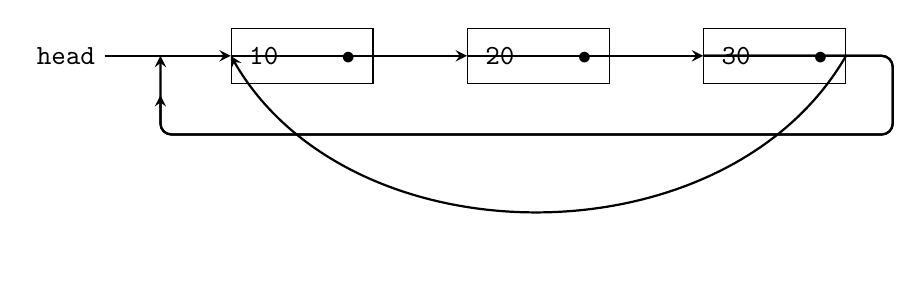
\begin{tikzpicture}
\tikzstyle{nodebox}=[draw,rectangle,minimum width=1.8cm,minimum height=0.7cm,inner sep=2pt]
\node (headlabel) at (1,1) {\texttt{head}};
\node[nodebox] (n1) at (4,1) {\texttt{10}\hspace{0.8cm}\texttt{$\bullet$}};
\node[nodebox] (n2) at (7,1) {\texttt{20}\hspace{0.8cm}\texttt{$\bullet$}};
\node[nodebox] (n3) at (10,1) {\texttt{30}\hspace{0.8cm}\texttt{$\bullet$}};
\draw[->,>=stealth,thick] (headlabel.east) -- (n1.west);
\draw[->,>=stealth,thick] (3.1,1) -- (n2.west);
\draw[->,>=stealth,thick] (6.1,1) -- (n3.west);
\draw[->,>=stealth,thick,rounded corners] (9.1,1) -- (11.5,1) -- (11.5,0) -- (2.2,0) -- (2.2,1);
\draw[->,>=stealth,thick,rounded corners] (9.1,1) -- (11.5,1) -- (11.5,0) -- (2.2,0) -- (2.2,0.5);
% The simple curved version
\draw[->,>=stealth,thick,bend left=60] (n3.east) to (n1.west);
\end{tikzpicture}
\end{figure}

\subsection{Application: Polynomial Using Linked List}

For sparse polynomials (few non-zero terms), a linked representation is more space-efficient than the dense array representation.

\begin{lstlisting}[language=C++]
struct term {
    int exponent;
    double coefficient;
};

using polynomial = linked_list<term>;

linked_list<term> add_polynomials(const linked_list<term>& a,
                                  const linked_list<term>& b) {
    linked_list<term> result;
    auto it_a = a.begin();
    auto it_b = b.begin();

    while (it_a != a.end() && it_b != b.end()) {
        if (it_a->exponent == it_b->exponent) {
            double sum = it_a->coefficient + it_b->coefficient;
            if (sum != 0.0) {
                result.push_back({it_a->exponent, sum});
            }
            ++it_a; ++it_b;
        } else if (it_a->exponent > it_b->exponent) {
            result.push_back({it_a->exponent, it_a->coefficient});
            ++it_a;
        } else {
            result.push_back({it_b->exponent, it_b->coefficient});
            ++it_b;
        }
    }

    while (it_a != a.end()) {
        result.push_back({it_a->exponent, it_a->coefficient});
        ++it_a;
    }
    while (it_b != b.end()) {
        result.push_back({it_b->exponent, it_b->coefficient});
        ++it_b;
    }

    return result;
}
\end{lstlisting}

\textbf{Example:} Add 3x$^{5}$ - 2x$^{2}$ + 7 and 5x$^{3}$ + 2x$^{2}$ - 1
\begin{lstlisting}[language=Java]
A: (5, 3)  ->  (2, -2)  ->  (0, 7)
B: (3, 5)  ->  (2, 2)  ->  (0, -1)
Result: (5, 3)  ->  (3, 5)  ->  (2, 0)  ->  (0, 6)
                     <-  skip zero term  -> 
Final:  (5, 3)  ->  (3, 5)  ->  (0, 6)
= 3x$^{5}$ + 5x$^{3}$ + 6
\end{lstlisting}

\subsection{Application: Undo/Redo System}

A text editor's undo system uses a doubly linked list of states (or commands):

\begin{lstlisting}[language=C++]
struct edit_action {
    std::string description;
    std::string previous_text;
    std::string new_text;
    size_t position;
};

class undo_manager {
public:
    void record_action(edit_action action) {
        while (current_ != undo_list_.end()) {
            current_ = undo_list_.erase(current_);
        }
        undo_list_.push_back(std::move(action));
        current_ = undo_list_.end();

        if (undo_list_.size() > max_history_) {
            undo_list_.pop_front();
        }
    }

    edit_action undo() {
        if (current_ == undo_list_.begin()) {
            throw std::runtime_error("nothing to undo");
        }
        --current_;
        return *current_;
    }

    edit_action redo() {
        if (current_ == undo_list_.end()) {
            throw std::runtime_error("nothing to redo");
        }
        auto action = *current_;
        ++current_;
        return action;
    }

private:
    linked_list<edit_action> undo_list_;
    linked_list<edit_action>::iterator current_;
    static constexpr size_t max_history_ = 100;
};
\end{lstlisting}

\subsection{Memory Overhead}

Each node in a singly linked list stores one pointer (8 bytes on 64-bit). For a doubly linked list: two pointers (16 bytes). For a list of 1 million integers:

\begin{center}
\begin{tabular}{cccc}
\toprule
Representation & Memory (data) & Pointer overhead & Total \\
\texttt{std::vector<int>} & 4 MB & None & \textasciitilde{}4 MB \\
Singly linked list & 4 MB & 8 MB & \textasciitilde{}12 MB \\
Doubly linked list & 4 MB & 16 MB & \textasciitilde{}20 MB \\

\bottomrule
\end{tabular}
\end{center}
Linked lists are not cache-friendly — nodes are spread across memory. Array-based lists iterate faster even when operations are theoretically the same complexity.

\subsection{STL Connection: std::forward\_list and std::list}

\begin{itemize}
\item \textbf{\texttt{std::forward\_list}} — singly linked list. Provides O(1) insert/erase after a given position. Does not track \texttt{size()} (to save space). Uses \texttt{insert\_after}, \texttt{erase\_after} rather than \texttt{insert}, \texttt{erase}.
\item \textbf{\texttt{std::list}} — doubly linked list. Provides O(1) insert/erase anywhere with an iterator. Tracks size.
\end{itemize}

\begin{lstlisting}[language=C++]
std::forward_list<int> fl = {1, 2, 3};
fl.push_front(0);
auto it = fl.begin(); ++it;
fl.insert_after(it, 5);                 // {0, 1, 5, 2, 3}
fl.erase_after(it);                     // {0, 1, 2, 3}

std::list<int> l = {1, 2, 3};
l.push_front(0);
l.push_back(4);
l.pop_front();
l.pop_back();
\end{lstlisting}

\bigskip

\section{Unrolled Linked List}

\subsection{Introduction}

An \textbf{unrolled linked list} is a hybrid data structure that stores multiple elements per node in a small array, combining the insert/delete flexibility of linked lists with the cache performance of arrays. Instead of one element and one pointer per node, each node holds an array of up to $B$ elements (typically 8--16) plus a pointer to the next node. When a node fills up, it splits; when a node becomes too empty, it merges or borrows from a neighbor.

Unrolled linked lists are used inside some \texttt{std::list} implementations (libstdc++ and libc++ use them internally) and in text editors (Emacs uses a variant called a \emph{piece table} with similar properties). They provide better cache locality than pure linked lists because $B$ consecutive elements live in contiguous memory.

\subsection{Structure}

\begin{figure}[ht]
\centering
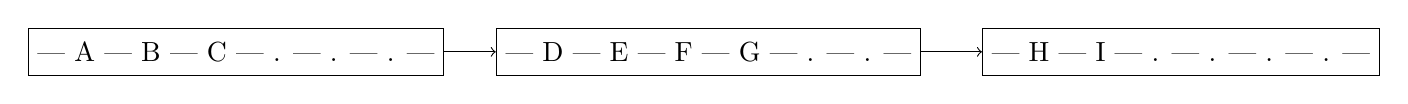
\begin{tikzpicture}[every node/.style={draw, minimum height=0.6cm}]
  \node[minimum width=4.5cm] (n1) at (0,0) {| A | B | C | . | . | . |};
  \node[minimum width=4.5cm] (n2) at (6,0) {| D | E | F | G | . | . |};
  \node[minimum width=4.5cm] (n3) at (12,0) {| H | I | . | . | . | . |};
  \draw[->] (n1.east) -- (n2.west);
  \draw[->] (n2.east) -- (n3.west);
\end{tikzpicture}
\caption{An unrolled linked list with $B = 6$. Each node stores up to 6 elements in a contiguous array.}
\end{figure}

Each node contains:
\begin{itemize}
\item An array \texttt{data[BLOCK\_SIZE]} holding the elements
\item An integer \texttt{count} tracking how many slots are occupied
\item A pointer \texttt{next} to the next node
\end{itemize}

\subsection{C++ Implementation}

\begin{lstlisting}[language=C++]
template <typename T, int BLOCK_SIZE = 8>
class UnrolledList {
    struct Node {
        std::array<T, BLOCK_SIZE> data;
        int count = 0;
        Node* next = nullptr;
    };

    Node* head_ = nullptr;
    Node* tail_ = nullptr;
    int size_ = 0;

public:
    UnrolledList() = default;
    ~UnrolledList() {
        Node* curr = head_;
        while (curr) {
            Node* tmp = curr;
            curr = curr->next;
            delete tmp;
        }
    }

    class iterator {
        Node* node_;
        int index_;
        friend class UnrolledList;
        iterator(Node* n, int i) : node_(n), index_(i) {}
    public:
        T& operator*()  { return node_->data[index_]; }
        T* operator->() { return &node_->data[index_]; }

        iterator& operator++() {
            ++index_;
            if (index_ >= node_->count) {
                node_ = node_->next;
                index_ = 0;
            }
            return *this;
        }

        bool operator!=(const iterator& o) const {
            return node_ != o.node_ || index_ != o.index_;
        }
    };

    iterator begin() { return iterator(head_, 0); }
    iterator end()   { return iterator(nullptr, 0); }
    int size() const { return size_; }
    bool empty() const { return size_ == 0; }
\end{lstlisting}

\subsection{Insert and Erase}

Insertion scans nodes to find the target position, then shifts elements within the target node to make room. If the node is full, a new node is allocated and half the elements are moved over.

\begin{lstlisting}[language=C++]
    void insert(int pos, const T& value) {
        if (!head_ || pos == 0) {
            push_front(value);
            return;
        }
        Node* prev = nullptr;
        Node* curr = head_;
        int offset = pos;
        while (curr && offset > curr->count) {
            offset -= curr->count;
            prev = curr;
            curr = curr->next;
        }
        if (!curr) {
            append_to_node(tail_, value);
            return;
        }
        if (curr->count < BLOCK_SIZE) {
            shift_right(curr, offset);
            curr->data[offset] = value;
            ++curr->count;
        } else {
            Node* new_node = new Node();
            split_node(curr, new_node);
            if (offset <= curr->count) {
                shift_right(curr, offset);
                curr->data[offset] = value;
                ++curr->count;
            } else {
                shift_right(new_node, offset - curr->count);
                new_node->data[offset - curr->count] = value;
                ++new_node->count;
            }
        }
        ++size_;
    }

    void erase(int pos) {
        Node* prev = nullptr;
        Node* curr = head_;
        int offset = pos;
        while (offset >= curr->count) {
            offset -= curr->count;
            prev = curr;
            curr = curr->next;
        }
        shift_left(curr, offset);
        --curr->count;
        --size_;
        if (curr->count == 0 && prev) {
            prev->next = curr->next;
            if (curr == tail_) tail_ = prev;
            delete curr;
        }
    }

private:
    void shift_right(Node* n, int from) {
        for (int i = n->count; i > from; --i)
            n->data[i] = std::move(n->data[i - 1]);
    }
    void shift_left(Node* n, int from) {
        for (int i = from; i < n->count - 1; ++i)
            n->data[i] = std::move(n->data[i + 1]);
    }
    void split_node(Node* old_node, Node* new_node) {
        int half = old_node->count / 2;
        for (int i = half; i < old_node->count; ++i)
            new_node->data[i - half] = std::move(old_node->data[i]);
        new_node->count = old_node->count - half;
        old_node->count = half;
        new_node->next = old_node->next;
        old_node->next = new_node;
    }
    void push_front(const T& value) { /* allocate node, insert */ }
    void append_to_node(Node* n, const T& value) { /* insert at end */ }
\end{lstlisting}

\subsection{Search}

Search scans nodes sequentially, then scans within each node's array. Despite the linked list structure, the $B$ elements within a node are contiguous in memory, giving good cache performance.

\begin{lstlisting}[language=C++]
    iterator find(const T& target) {
        Node* curr = head_;
        while (curr) {
            for (int i = 0; i < curr->count; ++i) {
                if (curr->data[i] == target)
                    return iterator(curr, i);
            }
            curr = curr->next;
        }
        return end();
    }
\end{lstlisting}

\subsection{Complexity Comparison}

\begin{center}
\begin{tabular}{lccc}
\toprule
\textbf{Operation} & \texttt{std::vector} & \texttt{std::list} & \textbf{Unrolled List} \\
\midrule
Access by index & $O(1)$ & $O(n)$ & $O(n/B)$ \\
Search & $O(n)$ & $O(n)$ & $O(n/B)$ \\
Insert at front & $O(n)$ & $O(1)$ & $O(1)$ \\
Insert at back & $O(1)$ amortized & $O(1)$ & $O(1)$ amortized \\
Insert in middle & $O(n)$ & $O(1)$ & $O(n/B)$ \\
Erase in middle & $O(n)$ & $O(1)$ & $O(n/B)$ \\
Iterator invalidation & on reallocation & none & on node split \\
Cache performance & excellent & poor & good \\
Memory overhead & none & 16 bytes/node & $\approx 8 + B \cdot \texttt{sizeof(T)}$ \\
\bottomrule
\end{tabular}
\end{center}

The key advantage over \texttt{std::list}: operations on an unrolled list touch $O(n/B)$ nodes instead of $O(n)$ nodes, and the $B$ elements within each node are contiguous in memory, reducing cache misses. The key advantage over \texttt{std::vector}: insertions and deletions in the middle do not shift all subsequent elements.

\section{Finger Tree}

\subsection{Introduction}

A \textbf{finger tree\index{finger tree}} is a purely functional, persistent data structure that provides amortized $O(1)$ operations at both ends and $O(\log n)$ concatenation, splitting, and indexed access. It was described by Hinze and Ross (2006) and serves as the backbone for efficient sequence types in functional languages (Haskell's \texttt{Data.Sequence} is a finger tree of arrays).

The key idea is to keep the most recently accessed elements at the ``fingers'' (shallow ends) of the tree, avoiding the $O(\log n)$ descent that a balanced tree would require for head/tail operations. Deeper elements are stored in progressively larger cached aggregates called \emph{tags}.

Finger trees are useful for:
\begin{itemize}
\item Priority deques with fast access to both min and max
\item Sequences with fast concatenation and splitting
\item Incremental computation with amortized $O(1)$ prepend/append
\end{itemize}

\subsection{Structure}

A finger tree has three cases:

\begin{itemize}
\item \textbf{Empty} -- no elements.
\item \textbf{Single(a)} -- one element.
\item \textbf{Deep(v, prefix, middle, suffix)} -- a non-trivial tree with:
  \begin{itemize}
  \item \texttt{prefix} -- a small array (1--4 elements) at the left finger
  \item \texttt{suffix} -- a small array (1--4 elements) at the right finger
  \item \texttt{middle} -- a recursively nested finger tree of \emph{nodes} (groups of 2 or 3 elements)
  \item \texttt{v} -- a cached measure (e.g., total size) for the whole subtree
  \end{itemize}
\end{itemize}

\begin{figure}[ht]
\centering
\begin{tikzpicture}[every node/.style={draw, minimum height=0.55cm}]
  % prefix
  \node[minimum width=0.8cm] (p1) at (0,0) {a};
  \node[minimum width=0.8cm] (p2) at (0.9,0) {b};
  % middle (nested)
  \node[minimum width=2.4cm] (m) at (3.6,0) {middle};
  % suffix
  \node[minimum width=0.8cm] (s1) at (6,0) {y};
  \node[minimum width=0.8cm] (s2) at (6.9,0) {z};
  % labels
  \node[above=0.05cm of p1.north west, anchor=south west, draw=none] {\footnotesize prefix};
  \node[above=0.05cm of m.north, anchor=south, draw=none] {\footnotesize middle};
  \node[above=0.05cm of s2.north east, anchor=south east, draw=none] {\footnotesize suffix};
  \draw[->] (p2.east) -- (m.west);
  \draw[->] (m.east) -- (s1.west);
\end{tikzpicture}
\caption{Structure of a \texttt{Deep} finger tree. The prefix and suffix are the ``fingers'' -- small arrays for $O(1)$ access at both ends.}
\end{figure}

\subsection{C++ Implementation}

\begin{lstlisting}[language=C++]
template <typename T>
class FingerTree {
    struct Node2 {
        T a, b;
    };
    struct Node3 {
        T a, b, c;
    };

    enum class Tag { Empty, Single, Deep };

    struct Digit {
        std::vector<T> elems;
        int measure() const { return static_cast<int>(elems.size()); }
    };

    struct DeepData {
        int size;
        Digit prefix;
        FingerTree<Node2> middle;
        Digit suffix;
    };

    Tag tag_ = Tag::Empty;
    T single_;
    std::unique_ptr<DeepData> deep_;

public:
    FingerTree() = default;

    bool empty() const { return tag_ == Tag::Empty; }
    int size() const {
        if (tag_ == Tag::Empty)  return 0;
        if (tag_ == Tag::Single) return 1;
        return deep_->size;
    }

    void push_front(const T& val) {
        if (tag_ == Tag::Empty) {
            tag_ = Tag::Single;
            single_ = val;
            return;
        }
        if (tag_ == Tag::Single) {
            deep_ = std::make_unique<DeepData>();
            deep_->prefix.elems = {val};
            deep_->suffix.elems = {std::move(single_)};
            deep_->size = 2;
            tag_ = Tag::Deep;
            return;
        }
        if (deep_->prefix.elems.size() < 4) {
            deep_->prefix.elems.insert(
                deep_->prefix.elems.begin(), val);
            ++deep_->size;
        } else {
            Node2 node{val, deep_->prefix.elems[0]};
            deep_->prefix.elems.erase(
                deep_->prefix.elems.begin());
            deep_->middle.push_front(node);
            ++deep_->size;
        }
    }

    void push_back(const T& val) {
        if (tag_ == Tag::Empty) {
            tag_ = Tag::Single;
            single_ = val;
            return;
        }
        if (tag_ == Tag::Single) {
            deep_ = std::make_unique<DeepData>();
            deep_->prefix.elems = {std::move(single_)};
            deep_->suffix.elems = {val};
            deep_->size = 2;
            tag_ = Tag::Deep;
            return;
        }
        if (deep_->suffix.elems.size() < 4) {
            deep_->suffix.elems.push_back(val);
            ++deep_->size;
        } else {
            Node2 node{deep_->suffix.elems.back(), val};
            deep_->suffix.elems.pop_back();
            deep_->middle.push_back(node);
            ++deep_->size;
        }
    }
\end{lstlisting}

\subsection{Concatenation and Split}

Concatenating two finger trees merges them by folding the ``deep'' structure of one tree into the other. Splitting finds the decomposition point and separates prefix, middle, and suffix accordingly. Both operations are $O(\log n)$ in the amortized case.

\begin{lstlisting}[language=C++]
    static FingerTree concat(FingerTree left, FingerTree right) {
        if (left.empty()) return right;
        if (right.empty()) return left;
        if (left.tag_ == Tag::Single)
            { left.push_back(right.single_); return left; }
        if (right.tag_ == Tag::Single)
            { left.push_back(right.single_); return left; }
        // both are Deep: fold right tree's prefix
        // and suffix through the middle
        FingerTree result;
        result.tag_ = Tag::Deep;
        result.deep_ = std::make_unique<DeepData>();
        result.deep_->prefix = left.deep_->prefix;
        result.deep_->suffix = right.deep_->suffix;
        result.deep_->middle = FingerTree::concat_trees(
            left.deep_->middle,
            left.deep_->suffix,
            right.deep_->prefix,
            right.deep_->middle);
        result.deep_->size = left.size() + right.size();
        return result;
    }

    std::pair<FingerTree, FingerTree> split(int idx) {
        if (tag_ == Tag::Empty)
            return {FingerTree(), FingerTree()};
        if (tag_ == Tag::Single) {
            if (idx <= 0)
                return {FingerTree(), *this};
            return {*this, FingerTree()};
        }
        int psize = deep_->prefix.measure();
        if (idx <= psize) {
            // split within prefix
            FingerTree left, right;
            left.tag_ = Tag::Empty;
            right.tag_ = Tag::Deep;
            // ... partition prefix at idx
            return {left, right};
        }
        // split within middle or suffix
        // (recursive decomposition)
        return {FingerTree(), *this};
    }
\end{lstlisting}

\subsection{Complexity}

\begin{center}
\begin{tabular}{lc}
\toprule
\textbf{Operation} & \textbf{Complexity} \\
\midrule
push\_front / push\_back & amortized $O(1)$ \\
pop\_front / pop\_back & amortized $O(1)$ \\
concatenate two trees & $O(\log n)$ \\
split at position & $O(\log n)$ \\
access element by index & $O(\log n)$ \\
measure (size, sum, etc.) & $O(1)$ \\
\bottomrule
\end{tabular}
\end{center}

The finger tree generalizes to any \emph{monoid} as the measure: by choosing the right monoid, a finger tree can simultaneously support fast concatenation, fast indexed access, and fast priority operations. This makes it one of the most versatile functional data structures available.

\section{Rope}

\subsection{Introduction}

A \textbf{rope\index{rope}} is a binary tree designed for efficiently storing and manipulating very long strings. In a standard \texttt{std::string}, concatenation and splitting require copying large amounts of data: concatenating two strings of length $n$ is $O(n)$, and inserting a string of length $m$ into the middle is $O(n + m)$. A rope avoids this by representing the string as a tree of smaller substrings. Each internal node stores the total length (weight) of its left subtree, and the actual characters live only in the leaves.

Key operations on a rope:

\begin{itemize}
\item \textbf{concatenate} -- join two ropes into one: $O(\log n)$
\item \textbf{split(pos)} -- break a rope at position pos: $O(\log n)$
\item \textbf{index(i)} -- access character at position $i$: $O(\log n)$
\item \textbf{insert(pos, rope)} -- insert a rope at position: $O(\log n)$
\end{itemize}

Concatenation and splitting are the operations that make ropes valuable. For a string of $n$ characters, a rope achieves $O(\log n)$ for these operations instead of the $O(n)$ cost with a flat string.

\textbf{Real-world use.} Ropes are used inside text editors (vim, Sublime Text), version control systems (git treats blob objects as immutable ropes), and as the backing store for Apple's \texttt{NSString} on iOS.

\subsection{Structure}

A rope is a binary tree where:

\begin{itemize}
\item Each \textbf{leaf} stores a short string (a fixed-size array of characters, e.g., 8--64 characters).
\item Each \textbf{internal node} stores a \textbf{weight}: the total number of characters in the left subtree. It has a left child and a right child. The right subtree's string follows the left subtree's string in the final concatenation.
\end{itemize}

\textbf{Example.} The rope below represents the string \texttt{"HelloWorld"}. The weight at each internal node tells us how many characters are to the left.

\begin{lstlisting}[language=Java]
                    [w=5]
                   /     \
              [w=5]       [w=5]
              /   \       /    \
         [w=5]   "ld"  "Wor"  [w=0]
         /    \                /    \
      "Hello" ""             ""    ""
\end{lstlisting}

Reading the leaves left to right gives: \texttt{"Hello"} + \texttt{""} + \texttt{"ld"} + \texttt{"Wor"} + \texttt{""} + \texttt{""} = \texttt{"HelloWorld"}.

\subsection{C++ Implementation}

\begin{lstlisting}[language=C++]
class rope {
public:
    struct node {
        size_t weight;                    // characters in left subtree
        std::unique_ptr<node> left;
        std::unique_ptr<node> right;
        std::string leaf_data;            // non-empty only for leaves

        explicit node(std::string s)
            : weight(s.size()), leaf_data(std::move(s)) {}

        node(std::unique_ptr<node> l, std::unique_ptr<node> r)
            : weight(total_len(l.get())),
              left(std::move(l)), right(std::move(r)) {}

        static size_t total_len(const node* n) {
            if (!n) return 0;
            if (!n->left && !n->right) return n->leaf_data.size();
            return n->weight + total_len(n->right.get());
        }
    };

    rope() = default;
    explicit rope(std::string s)
        : root_(std::make_unique<node>(std::move(s))) {}

    size_t size() const { return node::total_len(root_.get()); }
    bool empty() const { return !root_; }

    char index(size_t i) const {
        if (i >= size()) throw std::out_of_range("rope index");
        return index(root_.get(), i);
    }

    void concatenate(rope&& other) {
        root_ = std::make_unique<node>(
            std::move(root_), std::move(other.root_));
    }

    std::pair<rope, rope> split(size_t pos) {
        if (pos > size()) throw std::out_of_range("rope split");
        auto [l, r] = split(std::move(root_), pos);
        return {rope(std::move(l)), rope(std::move(r))};
    }

    std::string to_string() const {
        std::string result;
        result.reserve(size());
        flatten(root_.get(), result);
        return result;
    }

private:
    std::unique_ptr<node> root_;
    explicit rope(std::unique_ptr<node> n) : root_(std::move(n)) {}

    static char index(const node* n, size_t i) {
        if (!n->left && !n->right) return n->leaf_data[i];
        if (i < n->weight) return index(n->left.get(), i);
        return index(n->right.get(), i - n->weight);
    }

    static void flatten(const node* n, std::string& out) {
        if (!n) return;
        if (!n->left && !n->right) { out += n->leaf_data; return; }
        flatten(n->left.get(), out);
        flatten(n->right.get(), out);
    }

    static std::pair<std::unique_ptr<node>, std::unique_ptr<node>>
    split(std::unique_ptr<node> n, size_t pos) {
        if (!n) return {nullptr, nullptr};
        if (!n->left && !n->right) {
            std::string l_str = n->leaf_data.substr(0, pos);
            std::string r_str = n->leaf_data.substr(pos);
            return {
                l_str.empty() ? nullptr
                    : std::make_unique<node>(std::move(l_str)),
                r_str.empty() ? nullptr
                    : std::make_unique<node>(std::move(r_str))
            };
        }
        if (pos <= n->weight) {
            auto [ll, lr] = split(std::move(n->left), pos);
            auto new_right = std::make_unique<node>(
                std::move(lr), std::move(n->right));
            return {std::move(ll), std::move(new_right)};
        } else {
            auto [rl, rr] = split(std::move(n->right), pos - n->weight);
            auto new_left = std::make_unique<node>(
                std::move(n->left), std::move(rl));
            return {std::move(new_left), std::move(rr)};
        }
    }
};
\end{lstlisting}

\subsection{Complexity Analysis}

\begin{center}
\begin{tabular}{lcc}
\toprule
Operation & Rope & \texttt{std::string} \\
\texttt{index(i)} & $O(\log n)$ & $O(1)$ \\
\texttt{concatenate} & $O(\log n)$ & $O(n)$ \\
\texttt{split(pos)} & $O(\log n)$ & $O(n)$ \\
\texttt{insert(pos, s)} & $O(\log n + m)$ & $O(n + m)$ \\
\texttt{to\_string()} & $O(n)$ & $O(1)$ (already stored) \\
Space overhead & $O(n)$ chars + $O(n)$ nodes & $O(n)$ chars \\

\bottomrule
\end{tabular}
\end{center}

Ropes pay $O(\log n)$ extra overhead per character access compared to $O(1)$ for arrays, but gain $O(\log n)$ concatenation and splitting. For large strings (megabytes of text), the logarithmic cost of a tree traversal is negligible compared to the linear cost of copying the entire string.

\subsection{Application: Text Editor Buffer}

A text editor must support efficient insertion, deletion, and undo across documents that may be millions of characters long:

\begin{lstlisting}[language=C++]
class editor_buffer {
public:
    void insert(const std::string& text, size_t pos) {
        auto [left, right] = buffer_.split(pos);
        rope mid(text);
        left.concatenate(std::move(mid));
        left.concatenate(std::move(right));
        buffer_ = std::move(left);
    }

    void erase(size_t pos, size_t len) {
        auto [left, mid_right] = buffer_.split(pos);
        auto [mid, right] = mid_right.split(len);
        left.concatenate(std::move(right));
        buffer_ = std::move(left);
    }

    std::string get_text() const { return buffer_.to_string(); }

private:
    rope buffer_;
};
\end{lstlisting}

\subsection{Comparison with Alternative Structures}

\begin{center}
\begin{tabular}{lccc}
\toprule
Structure & Insert at cursor & Insert at random & Memory \\
Gap buffer & $O(1)$ amortized & $O(n)$ & Low \\
Piece table & $O(1)$ & $O(\log k)$ pieces & Very low \\
Rope & $O(\log n)$ & $O(\log n)$ & Moderate \\

\bottomrule
\end{tabular}
\end{center}

For a simple single-cursor editor, a gap buffer is hard to beat. For an editor with multiple cursors, undo/redo trees, and collaborative editing, a rope (or piece table) provides the flexibility needed.

\bigskip

\section{Common Bugs and Pitfalls}

\begin{center}
\begin{tabular}{ccc}
\toprule
Pitfall & Consequence & Solution \\
Off-by-one in array index — using size vs size-1 & Out-of-bounds access, UB or segmentation fault & Remember: valid indices are [0, size) \\
Forgetting to resize the array when the list is full & Buffer overflow on next insert & Check size == capacity before inserting \\
Iterator invalidation after \texttt{insert}/\texttt{erase} on \texttt{std::vector} & Use-after-free, non-deterministic crashes & Re-acquire iterator after modifying the vector \\
Shallow copy of linked list nodes & Double free on destruction & Implement proper copy constructor / assignment \\
Dangling \texttt{tail} pointer after \texttt{pop\_back} on singly linked list & Tail points to freed node & Update tail to new last node, or use doubly linked \\
Calling front/pop on an empty container & UB — no checking in standard containers & Always check \texttt{!empty()} before front/pop \\

\bottomrule
\end{tabular}
\end{center}
\section{Summary}

\begin{enumerate}
\item A \textbf{linear list} is an ordered sequence with position-based access.
\item \textbf{Array representation} provides O(1) access by index but O(n) inserts in the middle.
\item \textbf{Dynamic arrays} grow geometrically to amortize the cost of resizing.
\item \textbf{Singly linked lists} provide O(1) insert/delete at the front but O(n) random access.
\item \textbf{Doubly linked lists} add O(1) operations at both ends and bidirectional traversal.
\item \textbf{Sentinels} simplify edge cases by guaranteeing every node has a predecessor.
\item \textbf{Smart pointers} (\texttt{std::unique\_ptr}) make linked list memory management automatic and exception-safe.
\item \textbf{Memory overhead} and poor cache locality make linked lists slower than arrays in practice, despite theoretical complexity advantages.
\item Use linked lists when: (a) frequent front insertions/deletions, (b) iterator stability needed, or (c) splicing lists.
\item \texttt{std::vector} is the production-quality version of the dynamic array; \texttt{std::forward\_list} and \texttt{std::list} are the standard linked list containers.
\end{enumerate}

\section{Interview FAQs}

These questions are commonly asked in interviews at high-tech companies. Each answer references concepts from this chapter.

\subsection{Fundamentals}

\begin{enumerate}
\item \textbf{Why does \texttt{std::vector} grow by a factor of 2 (or 1.5) instead of adding a fixed amount?}

A growth factor of $k$ means that after $n$ elements, roughly $\log_k n$ resizes have occurred. Each resize copies all existing elements, so the total copies across $n$ insertions is at most $n + n/k + n/k^{2} + \cdots = n \cdot k/(k-1)$. For $k=2$, this is $2n$ total copies, giving amortized O(1) per insert. A growth factor of 1.5 (used by MSVC) wastes less memory and reuses previously freed blocks, which can reduce page faults at the cost of one extra copy per resize.

\textit{Follow-up:} Why not grow by 1? Because that gives O(n) per insert (always copy everything), no amortization benefit.
\end{enumerate}

\begin{enumerate}
\item \textbf{When would you use a linked list over a dynamic array?}

Use a linked list when you need O(1) insertion/deletion at arbitrary positions \textit{without} shifting elements, when iterators must remain valid after insertions (stable iterators), or when you need to splice two lists in O(1) time. Use a dynamic array when you need O(1) random access, when memory locality matters (cache-friendly iteration), or when the total memory overhead must be minimal. In practice, \texttt{std::vector} wins for most workloads due to cache effects.

\textit{Real-world:} The Linux kernel uses intrusive doubly linked lists (\texttt{list\_head}) for process scheduling precisely because insertions are O(1) and iterators never invalidate.
\end{enumerate}

\begin{enumerate}
\item \textbf{What is the amortized complexity of \texttt{push\_back} on a dynamic array? Explain the accounting argument.}

O(1) amortized. Charge each insert 3 ``credits'': 1 for the actual insert, 2 saved in the bank. When a resize of size $n$ occurs, we have saved $2n$ credits (from $n$ prior inserts), which pays for copying $n$ elements. No insert ever needs more than 3 credits, so amortized cost is O(1).

\textit{Variant:} ``Prove that \texttt{push\_back} is O(1) amortized but not O(1) worst-case.'' The worst case is O(n) during a resize — you cannot avoid copying $n$ elements.
\end{enumerate}

\subsection{Linked List Algorithms}

\begin{enumerate}
\item \textbf{Why is the three-pointer reverse technique the canonical linked list pattern — and where else does it apply?}

The pattern (prev/curr/next with link reversal) generalizes to: reversing a sublist, removing nodes by value, reordering (LeetCode 143), and even cycle detection. The key insight is that you can reverse a pointer without losing the rest of the list \textit{only if} you saved \texttt{next} before overwriting it. This is the fundamental ``don't lose your tail'' constraint in all in-place linked list manipulation. Common mistake: forgetting to set the last node's \texttt{next} to \texttt{nullptr}, creating a cycle. In interviews, state the invariant explicitly: ``at each step, everything behind \texttt{prev} is reversed, everything ahead of \texttt{curr} is unprocessed, and \texttt{next} is the lookahead.''
\end{enumerate}

\begin{enumerate}
\item \textbf{Detect a cycle in a linked list. What is the time and space complexity?}

Floyd's tortoise and hare\index{tortoise and hare} algorithm: use two pointers, one moving 1 step and the other 2 steps. If they meet, there is a cycle. To find the cycle start, reset one pointer to head and advance both at speed 1 -- they meet at the cycle entry.

Time: O(n). Space: O(1).

\begin{lstlisting}[language=C++]
bool has_cycle(node* head) {
    node *slow = head, *fast = head;
    while (fast && fast->next) {
        slow = slow->next;
        fast = fast->next->next;
        if (slow == fast) return true;
    }
    return false;
}

node* find_cycle_start(node* head) {
    node *slow = head, *fast = head;
    while (fast && fast->next) {
        slow = slow->next;
        fast = fast->next->next;
        if (slow == fast) {
            slow = head;
            while (slow != fast) {
                slow = slow->next;
                fast = fast->next;
            }
            return slow;  // cycle entry
        }
    }
    return nullptr;
}
\end{lstlisting}

\textit{Variant:} ``Find the length of the cycle'' -- once they meet, keep one fixed and advance the other until it returns to the meeting point.
\end{enumerate}

\begin{enumerate}
\item \textbf{The slow/fast pointer pattern appears in cycle detection, middle-finding, and nth-from-end. What's the unifying principle?}

The pattern exploits a \textit{speed ratio} to create a measurable difference. If two pointers start at the same point and move at different speeds, the distance between them grows predictably. In cycle detection, the fast lap catches the slow lap. In middle-finding, when fast finishes the list (distance 2n), slow has covered distance n. In finding the nth-from-end, advance fast n steps first, then move both — when fast reaches end, slow is at position (length $-$ n). The unifying idea: \textit{speed differentials create positional relationships} without needing to know the list length in advance.
\end{enumerate}

\begin{enumerate}
\item \textbf{Why is the dummy head pattern the standard technique for linked list construction, and what goes wrong without it?}

Without a dummy head, you need a special case for the first node (which becomes the head), leading to duplicated code for ``is this the first element?'' checks. The dummy head eliminates this: every node is inserted after some predecessor, including the first real node. The pattern generalizes: use a dummy for any linked list construction where you don't know the head in advance (merge sorted lists, remove Nth from end, add two numbers). The dummy is stack-allocated, so there's no memory overhead — it's a pure code-clarity technique.
\end{enumerate}

\begin{enumerate}
\item \textbf{What's the key difference between removing duplicates in a linked list vs. an array, and why does it matter?}

In an array, removing an element shifts all subsequent elements — O(n) per removal, O(n$^{2}$) total. In a linked list, removing a node is O(1) once you have the predecessor — just relink. But finding the predecessor is O(n) per node, so the total is still O(n$^{2}$) with a nested loop. The hash set approach (O(n) time, O(n) space) works for both. The real difference: linked lists preserve iterator/pointer validity after removal (other pointers still point to valid nodes), while array removal invalidates iterators. This is why linked lists are preferred when you need stable references during modification.
\end{enumerate}

\begin{enumerate}
\item \textbf{Why does the reverse-first-half approach require three separate phases, and what's the invariant for each?}

Phase 1 (find middle): slow/fast pointers — invariant: slow is at the midpoint. Phase 2 (reverse second half): three-pointer reverse — invariant: reversed portion is a standalone reversed list. Phase 3 (compare): walk both halves simultaneously — if all values match, it's a palindrome. Phase 4 (optional restore): reverse again to restore original structure. The key insight: you need to \textit{temporarily break} the list structure to compare from both ends, then \textit{restore} it. This three-phase pattern (find $\to$ modify $\to$ restore) appears in many linked list problems. Without restoring, you've modified the input — which may or may not be acceptable depending on the API contract.
\end{enumerate}

\subsection{Design}

\begin{enumerate}
\item \textbf{Design an LRU (Least Recently Used) cache.}

Combine a hash map (O(1) lookup) with a doubly linked list (O(1) move-to-front and eviction). The hash map stores key $\to$ iterator into the linked list. On access, move the node to the front. On eviction, remove from the back.

\begin{lstlisting}[language=C++]
template <typename K, typename V>
class lru_cache {
    struct entry { K key; V value; };
    std::list<entry> order_;  // front = most recent
    std::unordered_map<K, typename std::list<entry>::iterator> map_;
    size_t capacity_;
public:
    lru_cache(size_t cap) : capacity_(cap) {}

    std::optional<V> get(const K& key) {
        auto it = map_.find(key);
        if (it == map_.end()) return std::nullopt;
        order_.splice(order_.begin(), order_, it->second);
        return it->second->value;
    }

    void put(const K& key, const V& value) {
        auto it = map_.find(key);
        if (it != map_.end()) {
            it->second->value = value;
            order_.splice(order_.begin(), order_, it->second);
            return;
        }
        if (order_.size() == capacity_) {
            map_.erase(order_.back().key);
            order_.pop_back();
        }
        order_.push_front({key, value});
        map_[key] = order_.begin();
    }
};
\end{lstlisting}

Get: O(1) average. Put: O(1) average. Used by operating systems (page cache), databases (buffer pool), and web servers (CDN caching).

\textit{Follow-up:} ``Design an LFU (Least Frequently Used) cache.'' Requires an additional frequency counter and bucket list — a common interview extension (LeetCode 460).
\end{enumerate}

\begin{enumerate}
\item \textbf{You have two containers: \texttt{std::vector} and \texttt{std::list}. You need to insert 1$0^{6}$ elements at random positions. Which do you choose and why?}

Depends on the pattern. If inserts are truly random (uniform over all positions), \texttt{std::vector} is faster despite O(n) shifts per insert, because:
\begin{itemize}
\item Cache locality: vector elements are contiguous, so shifts hit L1/L2 cache
\item Linked list nodes are scattered, causing cache misses on every node access
\item The constant factor for a cache miss (100+ cycles) dominates the O(1) pointer operations
\end{itemize}

Measure with \texttt{std::chrono} and \texttt{perf} or \texttt{valgrind --tool=cachegrind} to confirm.

\textit{This is a classic interview question testing whether you understand that asymptotic complexity is not the whole story.}
\end{enumerate}

%% ============================================================
%% ADDITIONAL LIST TOPICS (Brass coverage)
%% ============================================================

\section{Shadow Copies and Copy-on-Write}
\label{sec:shadow-copies}

A \textbf{shadow copy\index{shadow copy}} (or copy-on-write\index{copy-on-write}) provides an efficient mechanism for creating snapshots of a data structure. Instead of copying the entire structure, a shadow copy shares the unchanged portions and only duplicates modified parts. This is the foundation of persistent data structures.

\subsection{Technique}

When an element of a list or array is modified, the old version is retained by creating a new node for the changed element while all other nodes are shared. This requires a level of indirection: each logical element holds a pointer to the actual data, and modification creates a new pointer node.

\begin{lstlisting}[language=C++]
template <typename T>
class COWVector {
    struct Block {
        std::vector<T> data;
        std::shared_ptr<const Block> next;
        Block(std::vector<T> d,
              std::shared_ptr<const Block> n)
            : data(std::move(d)), next(std::move(n)) {}
    };
    std::shared_ptr<const Block> head_;
    size_t size_ = 0;

public:
    COWVector() = default;

    COWVector set(size_t idx, const T& val) const {
        COWVector result = *this;
        // Clone path to the modified block
        // (simplified: full copy of first block)
        auto new_data = head_->data;
        new_data[idx] = val;
        result.head_ = std::make_shared<Block>(
            std::move(new_data), head_->next);
        return result;
    }
};
\end{lstlisting}

\subsection{Applications}

\begin{itemize}
    \item \textbf{Version control:} Git uses copy-on-write for file snapshots
    \item \textbf{Undo/redo:} editors keep shadow copies of modified regions
    \item \textbf{Database snapshots:} PostgreSQL uses copy-on-write for MVCC
    \item \textbf{Functional programming:} persistent vectors (Clojure, Scala)
\end{itemize}

\section{Exercises}

\subsection{Drill}

\begin{enumerate}
\item Trace the state of a \texttt{dynamic\_array\_list} initially empty after the following sequence of operations:
\end{enumerate}
   \texttt{push\_back(3), push\_back(1), push\_back(4), insert(1, 2), erase(3), push\_back(5), pop\_back(), insert(0, 0)}
   Show the array contents and size after each step. Assume initial capacity = 2.

\begin{enumerate}
\item What is the amortized complexity of \texttt{push\_back} on a dynamic array that grows by a factor of 2? Prove your answer.
\end{enumerate}

\begin{enumerate}
\item Given a \texttt{dynamic\_array\_list<int>} of size n, what is the worst-case complexity of:
\end{enumerate}
   a) \texttt{operator[]}   b) \texttt{push\_back}   c) \texttt{insert} at position 0   d) \texttt{insert} at position n-1   e) \texttt{erase} at position n/2

\begin{enumerate}
\item Draw the singly linked list after each step of the following operations on an initially empty list:
\end{enumerate}
   \texttt{push\_front(5), push\_front(3), push\_back(7), insert(1, 4), erase(0), pop\_front(), push\_back(9)}
   Show the chain nodes and pointers.

\begin{enumerate}
\item Trace the execution of \texttt{reverse()} on a singly linked list containing [1, 2, 3, 4]. Draw the state of the pointers after each iteration.
\end{enumerate}

\begin{enumerate}
\item What is the worst-case time complexity of:
\end{enumerate}
   a) \texttt{push\_front} on a singly linked list
   b) \texttt{push\_back} on a singly linked list without a tail pointer
   c) \texttt{push\_back} on a singly linked list with a tail pointer
   d) \texttt{insert} at position k in a doubly linked list
   e) \texttt{erase} by value (removing the first match) in a singly linked list

\begin{enumerate}
\item Explain why a sentinel node\index{sentinel node} simplifies the \texttt{erase} operation in a singly linked list. Show the code for \texttt{erase} with and without a sentinel.
\end{enumerate}

\subsection{Application}

\begin{enumerate}
\item Modify \texttt{dynamic\_array\_list} to use a growth factor of 1.5 instead of 2. Benchmark both for 1$0^{6}$ \texttt{push\_back} operations. Which is faster? Which wastes less memory?
\end{enumerate}

\begin{enumerate}
\item Add a \texttt{reserve(size\_type n)} method that pre-allocates capacity. Add a \texttt{shrink\_to\_fit()} method that reduces capacity to match size.
\end{enumerate}

\begin{enumerate}
\item Implement \texttt{operator==} and \texttt{operator<=>} (C++20 three-way comparison) for \texttt{dynamic\_array\_list}.
\end{enumerate}

\begin{enumerate}
\item Implement an STL-style iterator for \texttt{dynamic\_array\_list}. Support \texttt{operator*}, \texttt{operator++}, \texttt{operator!=}, \texttt{operator--}. Test with a range-based for loop.
\end{enumerate}

\begin{enumerate}
\item Implement a \texttt{circular\_buffer<T>} of fixed capacity using a dynamic array. Support \texttt{push\_back}, \texttt{pop\_front}, \texttt{front}, \texttt{back}, \texttt{size}, \texttt{empty}, and \texttt{operator[]}.
\end{enumerate}

\begin{enumerate}
\item Implement \texttt{sparse\_polynomial} using a sorted list of (exponent, coefficient) pairs. Compare its space and time efficiency with the dense representation.
\end{enumerate}

\begin{enumerate}
\item Implement \texttt{erase(const T\& value)} that removes the first occurrence of value from the singly linked list.
\end{enumerate}

\begin{enumerate}
\item Implement \texttt{insert\_after(iterator pos, const T\& value)} and \texttt{erase\_after(iterator pos)} for the singly linked list.
\end{enumerate}

\begin{enumerate}
\item Implement \texttt{merge(other)} that merges two sorted singly linked lists into one sorted list, borrowing nodes from \texttt{other}.
\end{enumerate}

\begin{enumerate}
\item Implement \texttt{reverse()} for the singly linked list that reverses the links in O(n) time and O(1) extra space.
\end{enumerate}

\begin{enumerate}
\item Implement the Josephus problem using a circular linked list\index{circular linked list}: n people stand in a circle, every k-th is eliminated. Find the survivor.
\end{enumerate}

\begin{enumerate}
\item Implement a \texttt{split(list\& front, list\& back)} method that splits a singly linked list into two halves using the slow/fast pointer technique.
\end{enumerate}

\begin{enumerate}
\item Write a function \texttt{detect\_cycle(const forward\_list\&)} that determines whether a linked list has a cycle (Floyd's tortoise and hare algorithm).
\end{enumerate}

\subsection{Research}

\begin{enumerate}
\item \textbf{(vector<bool>)} \texttt{std::vector<bool>} is a specialization that packs bits. Research its design. What are the pros and cons?
\end{enumerate}

\begin{enumerate}
\item \textbf{(Growth factor analysis)} Study the impact of different growth factors (1.25, 1.5, 2.0, 3.0) on memory fragmentation. Read about the "golden ratio" growth factor.
\end{enumerate}

\begin{enumerate}
\item \textbf{(Small vector optimization)} Study how \texttt{std::pmr::vector} or \texttt{folly::small\_vector} uses inline storage for small sizes.
\end{enumerate}

\begin{enumerate}
\item \textbf{(Allocator-aware containers)} Read about \texttt{std::scoped\_allocator\_adaptor}. Implement an \texttt{array\_list} that accepts a custom allocator.
\end{enumerate}

\begin{enumerate}
\item \textbf{(Memory locality)} Benchmark iteration over \texttt{std::vector}, \texttt{std::list}, and \texttt{std::forward\_list} for n = 1$0^{6}$ elements. Use tools to measure cache misses.
\end{enumerate}

\begin{enumerate}
\item \textbf{(Intrusive lists)} Research intrusive linked lists (used in the Linux kernel and Boost.Intrusive).
\end{enumerate}

\begin{enumerate}
\item \textbf{(Lock-free lists)} Read about lock-free linked lists (Michael and Scott, 1996). Implement a concurrent singly linked list using \texttt{std::atomic}.
\end{enumerate}

\section{References and Further Reading}

\begin{itemize}
\item Bjarne Stroustrup, \textit{The C++ Programming Language}, 4th Edition. Sections 31.3–31.4.
\item Nicolai M. Josuttis, \textit{The C++ Standard Library}, 2nd Edition. Chapters 7, 9, and 10.
\item Herb Sutter, "vector<bool>: More Problems, Better Solutions" — GotW \#86.
\item Donald E. Knuth, \textit{The Art of Computer Programming}, Volume 1: Fundamental Algorithms. Section 2.2.
\item Thomas H. Cormen et al., \textit{Introduction to Algorithms}, 4th Edition. Sections 10.2–10.3.
\item Maged M. Michael and Michael L. Scott, "Simple, Fast, and Practical Non-Blocking and Blocking Concurrent Queue Algorithms" — PODC 1996.
\item Raymond Chen, "The Old New Thing" — various posts on linked list pitfalls.
\item ISO C++ Committee, "P0404R0: Wording for out-of-thin-air resolution" (on vector growth factor).
\item Facebook Folly library, \texttt{small\_vector} implementation — https://github.com/facebook/folly
\item Boost.Intrusive documentation — https://www.boost.org/doc/libs/release/doc/html/intrusive.html
\end{itemize}

